\chapter{Summary and Outlook}\label{ch:5}

\begin{figure*}
	\centering
	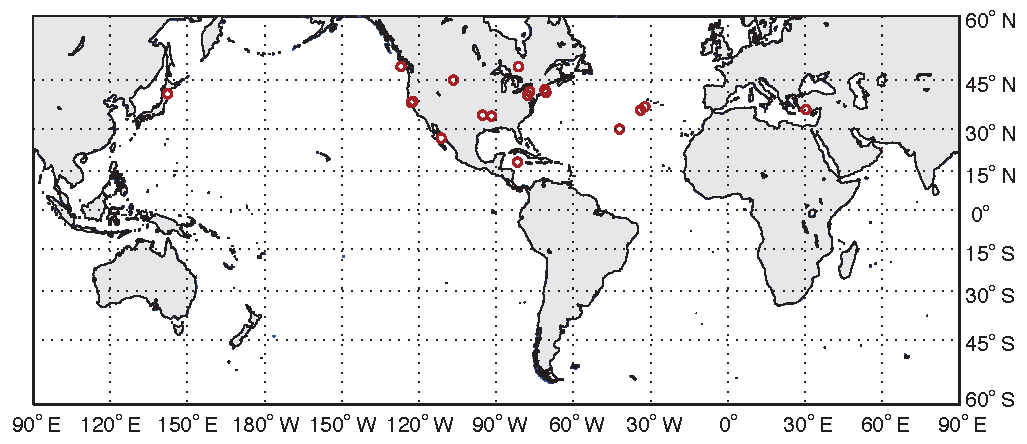
\includegraphics[width=\textwidth]{figures/Fig5.1.pdf}
	\captionsetup{format=myformat}	% hrule beneath caption
	\caption[Map of sample sites investigated by the MIT team]{Map showing locations of sites at which
		Δ\textsuperscript{13}CH\textsubscript{3}D measurements on samples have
		been published or presented from MIT.}
	\label{fig:5:1}
\end{figure*}

The preceding chapters presented a set of data (\autoref{fig:5:1}) that shows
several insights into the origin and fate of the methane stable
isotopologues in the environment. As of the time of writing, methane
clumped isotoplogue data have appeared in at least a dozen articles \parencite{Douglas++_2016_GCA,Stolper++_2014_GCA,Stolper++_2014_S,Stolper++_2015_GCA,Wang++_2015_S,Whitehill++_2017_GCA,Ono++_2014_AC,Wang++_2016_GCA,Lopes++_2016_JoDS,Inagaki++_2015_S,Young++_2016_IJMS,Young++_2017_GCA}.


\begin{SCfigure*}
	\centering
	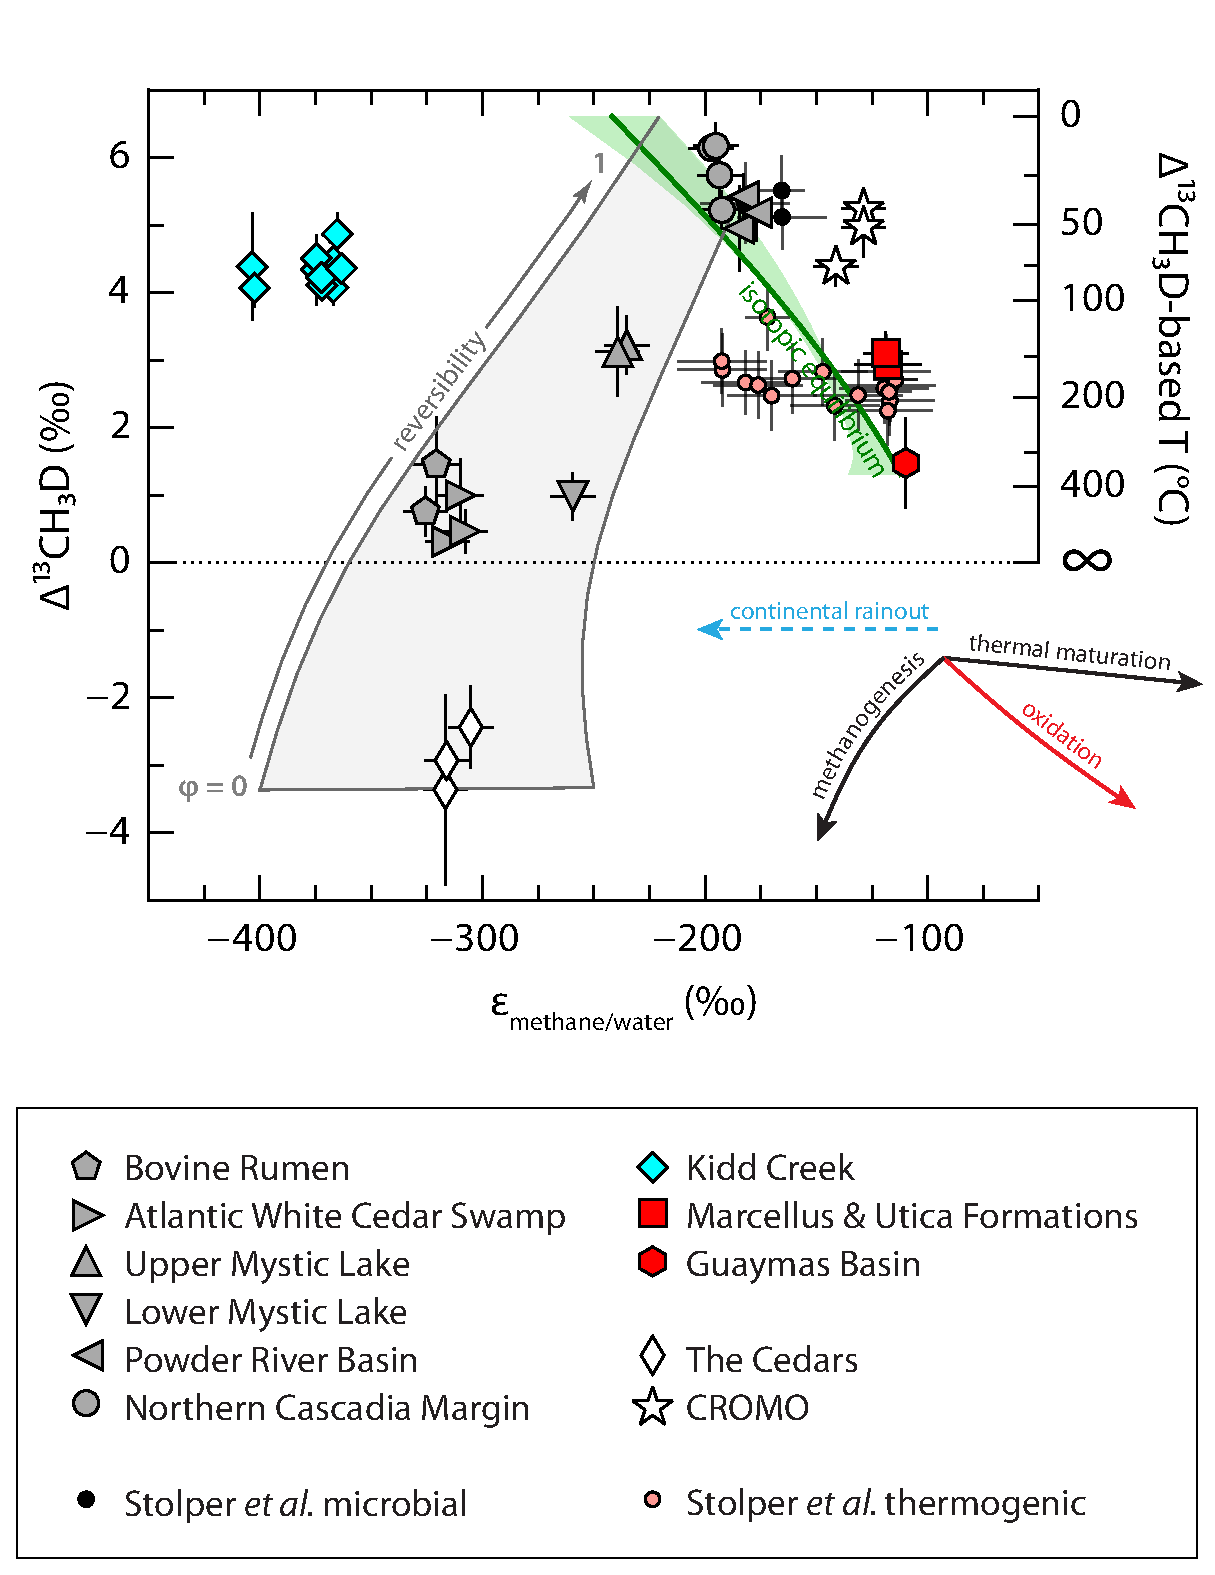
\includegraphics[width=0.57\textwidth]{figures/Fig5.2.pdf}
	\captionsetup{format=myformat}	% hrule beneath caption
	\caption[A survey of \textsuperscript{13}CH\textsubscript{3}D in the environment]{A survey of \textsuperscript{13}CH\textsubscript{3}D in
		the environment. This figure is the same as \autoref{fig:2:2}, with
		the addition of schematic vectors showing basic controls on the isotopic
		signatures of CH\textsubscript{4}, and data from \textcite{Stolper++_2014_S}.
		The position of their data along the \emph{x}-axis was calculated from
		estimated δD of formation waters, and for the \emph{y}-axis,
		Δ\textsubscript{18} values were converted to
		Δ\textsuperscript{13}CH\textsubscript{3}D by assuming equilibrium and
		applying the conversion shown in \mrefs[A]{Fig.}{fig:C:2}.}
	\label{fig:5:2}
\end{SCfigure*}

The Δ\textsuperscript{13}CH\textsubscript{3}D data were shown to be
independent of and complementary to δ\textsuperscript{13}C and δD. A
case was built for why hydrogen (or free energy) exerts a major control
on Δ\textsuperscript{13}CH\textsubscript{3}D and D/H of methane; this
and several other controls are shown in \autoref{fig:5:2}. And several
opportunities for advancement on the technical and theoretical sides of
the problem of methane origin have been highlighted (\autoref{fig:5:3}), including:
\begin{itemize}
	\item
	refining the calibration at low temperatures \parencite{Larson+Hall_1965_JPC,Naito++_2005_ApCat,Golden++_2001_JACS,Robertson++_1975_TFS};
	\item
	experiments to retrieve kinetics associated with the breaking and
	reforming of C--H bonds \parencite{Reeves++_2012_GCA,Lyon+Hulston_1984_GCA,Koepp_1978};
	\item
	construction of numerical models to test hypotheses regarding
	biophysical controls on isotopologue abundances.
\end{itemize}


\begin{figure*}
	\centering
	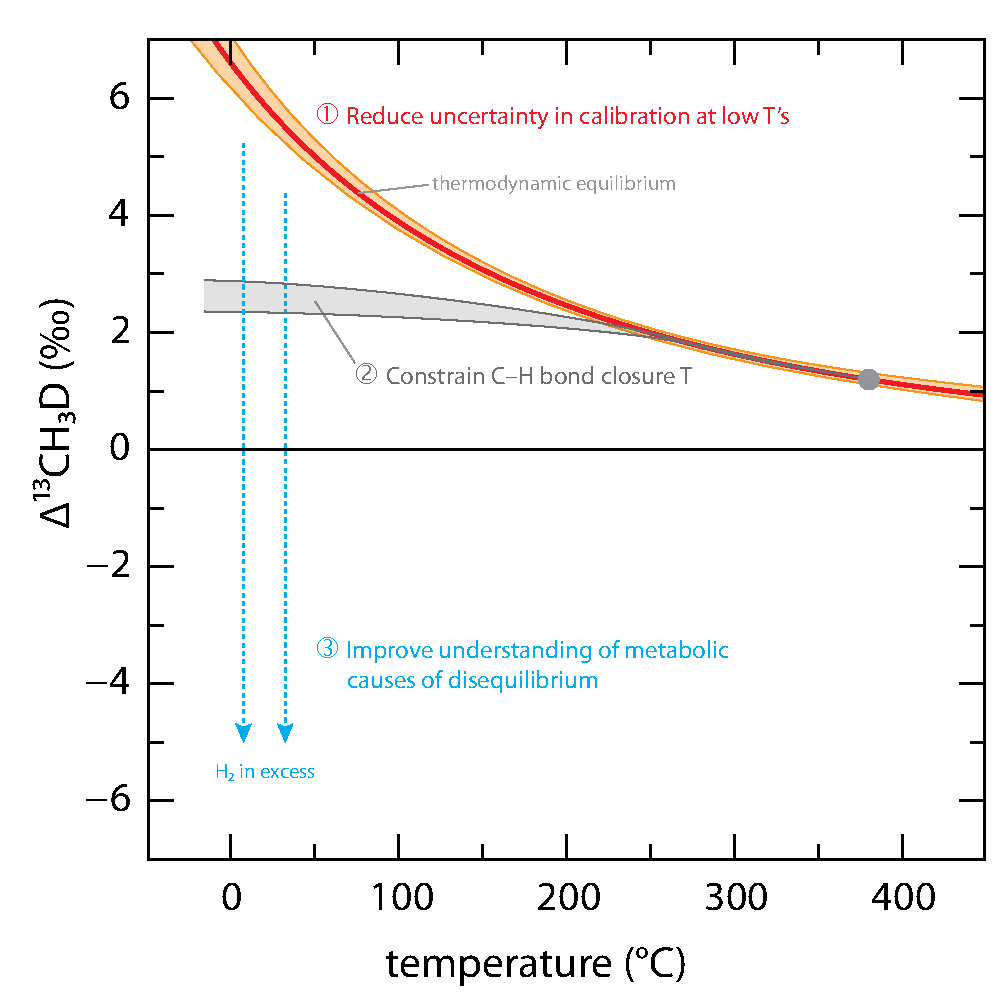
\includegraphics[width=0.5\textwidth]{figures/Fig5.3.pdf}
%	\captionsetup{format=myformat}	% hrule beneath caption
	\caption{Challenges and opportunities in understanding Δ\textsuperscript{13}CH\textsubscript{3}D}
	\label{fig:5:3}
\end{figure*}


Through this work, we have also realized that there is much more
information to be extracted from simple gas chemistry and conventional
stable isotope data than has perhaps been widely appreciated; or that
has been somewhat overlooked in the rush to develop and deploy new
technologies. Measurements of clumped isotopologues provide more
dimensions of data to characterize methane samples, which, as this
thesis shows, does provide additional constraints on certain Earth
systems. However, instruments to measure the doubly-substituted
isotopologues will likely remain a novelty for the foreseeable future.

I suspect that the most significant advances for our understanding of
the origins, transport, and fate of methane are still yet to come. The
biggest steps forward will come with moving away from straightforward
but often restrictive phenomenological representations of legacy data
and towards predictive and quantitative approaches to testing of
well-defined and geologically-plausible hypotheses. Isotopologue data
will certainly play a large role in helping narrow the solution space of
problems of geochemical nature. \mrefs[]{Figures}{fig:5:4} and \ref{fig:5:5} show some attempts at
making such data more easily accessible.


\begin{SCfigure*}
	\centering
	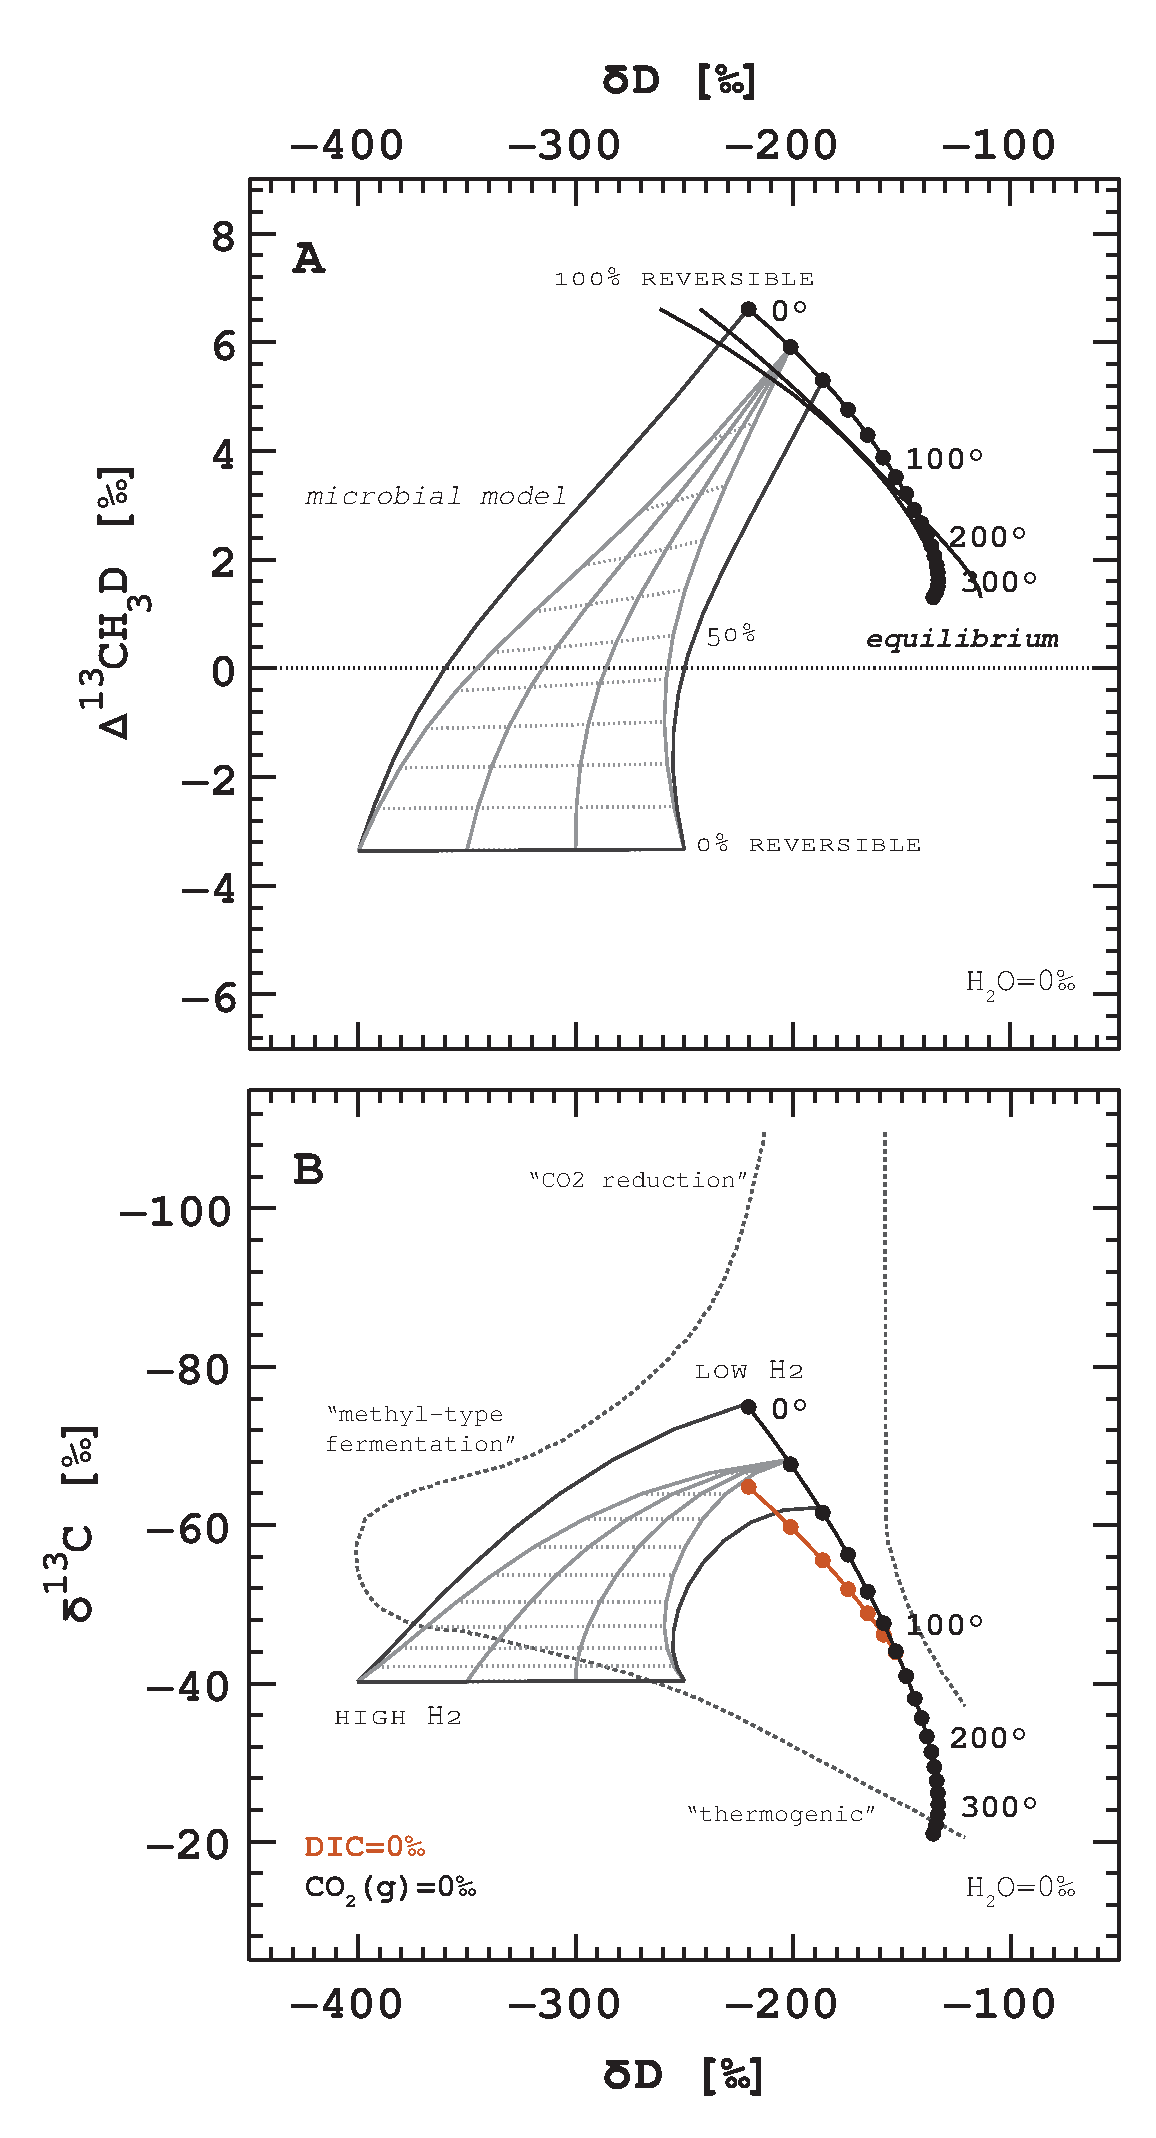
\includegraphics[scale=0.42]{figures/Fig5.4.pdf}
%	\captionsetup{format=myregular}	% no hrule beneath caption
	\caption[Predicted ratios of CH\textsubscript{4} isotopologues
	produced during hydrogenotrophic methanogenesis]{Model of isotopologue abundances in CH\textsubscript{4}
		produced during microbial methanogenesis from
		CO\textsubscript{2}+H\textsubscript{2} \parencite{Wang++_2015_S}. The model
		trajectories begin from a fully-reversible (equilibrium) line whose
		position is determined by assuming δ\textsuperscript{13}C of DIC or
		CO\textsubscript{2} are 0‰ vs.\ PDB. (This assumption is easily changed
		if, for example CO\textsubscript{2} has a higher
		\textsuperscript{13}C/\textsuperscript{12}C ratio than PDB.) The
		underlay in (B) is the outline of the frequently-used plot from \textcite{Whiticar_1990_OG}.
		
		\quad The plot indicates that modeled isotopic compositions for the
		fully-kinetic endmember are enriched in \textsuperscript{13}C and
		depleted in D relative to the equilibrium endmember. The fully-kinetic
		endmember is related to high H\textsubscript{2} concentrations (which
		yield a very large (negative) Δ\textsubscript{r}\emph{G}) \parencite{Burke_1993_Chemosphere}.
		Therefore, hydrogenotrophic methanogens could produce
		CH\textsubscript{4} with isotopic signatures indistinguishable from
		those typically attributed to methylotrophic or acetoclastic
		methanogenesis \parencite{Whiticar_1990_OG,Vinson++_2017_CG}. Whether this is
		true will require evaluation by experiments under low H\textsubscript{2}
		conditions \parencite{Valentine++_2004_GCA,Kawagucci++_2014_GCA,Okumura++_2016_ProgEPS} or \emph{in vitro} \parencite{Scheller++_2013_JACS_KIE}. Caveats to this
		model include (\emph{i}) the assumed fractionation factors may not
		approximate reality well, and (\emph{ii}) the possibility that the
		H-addition steps involved in methanogenesis may be differentially
		reversible in nature.}
	\label{fig:5:4}
\end{SCfigure*}



\begin{figure*}
	\centering
	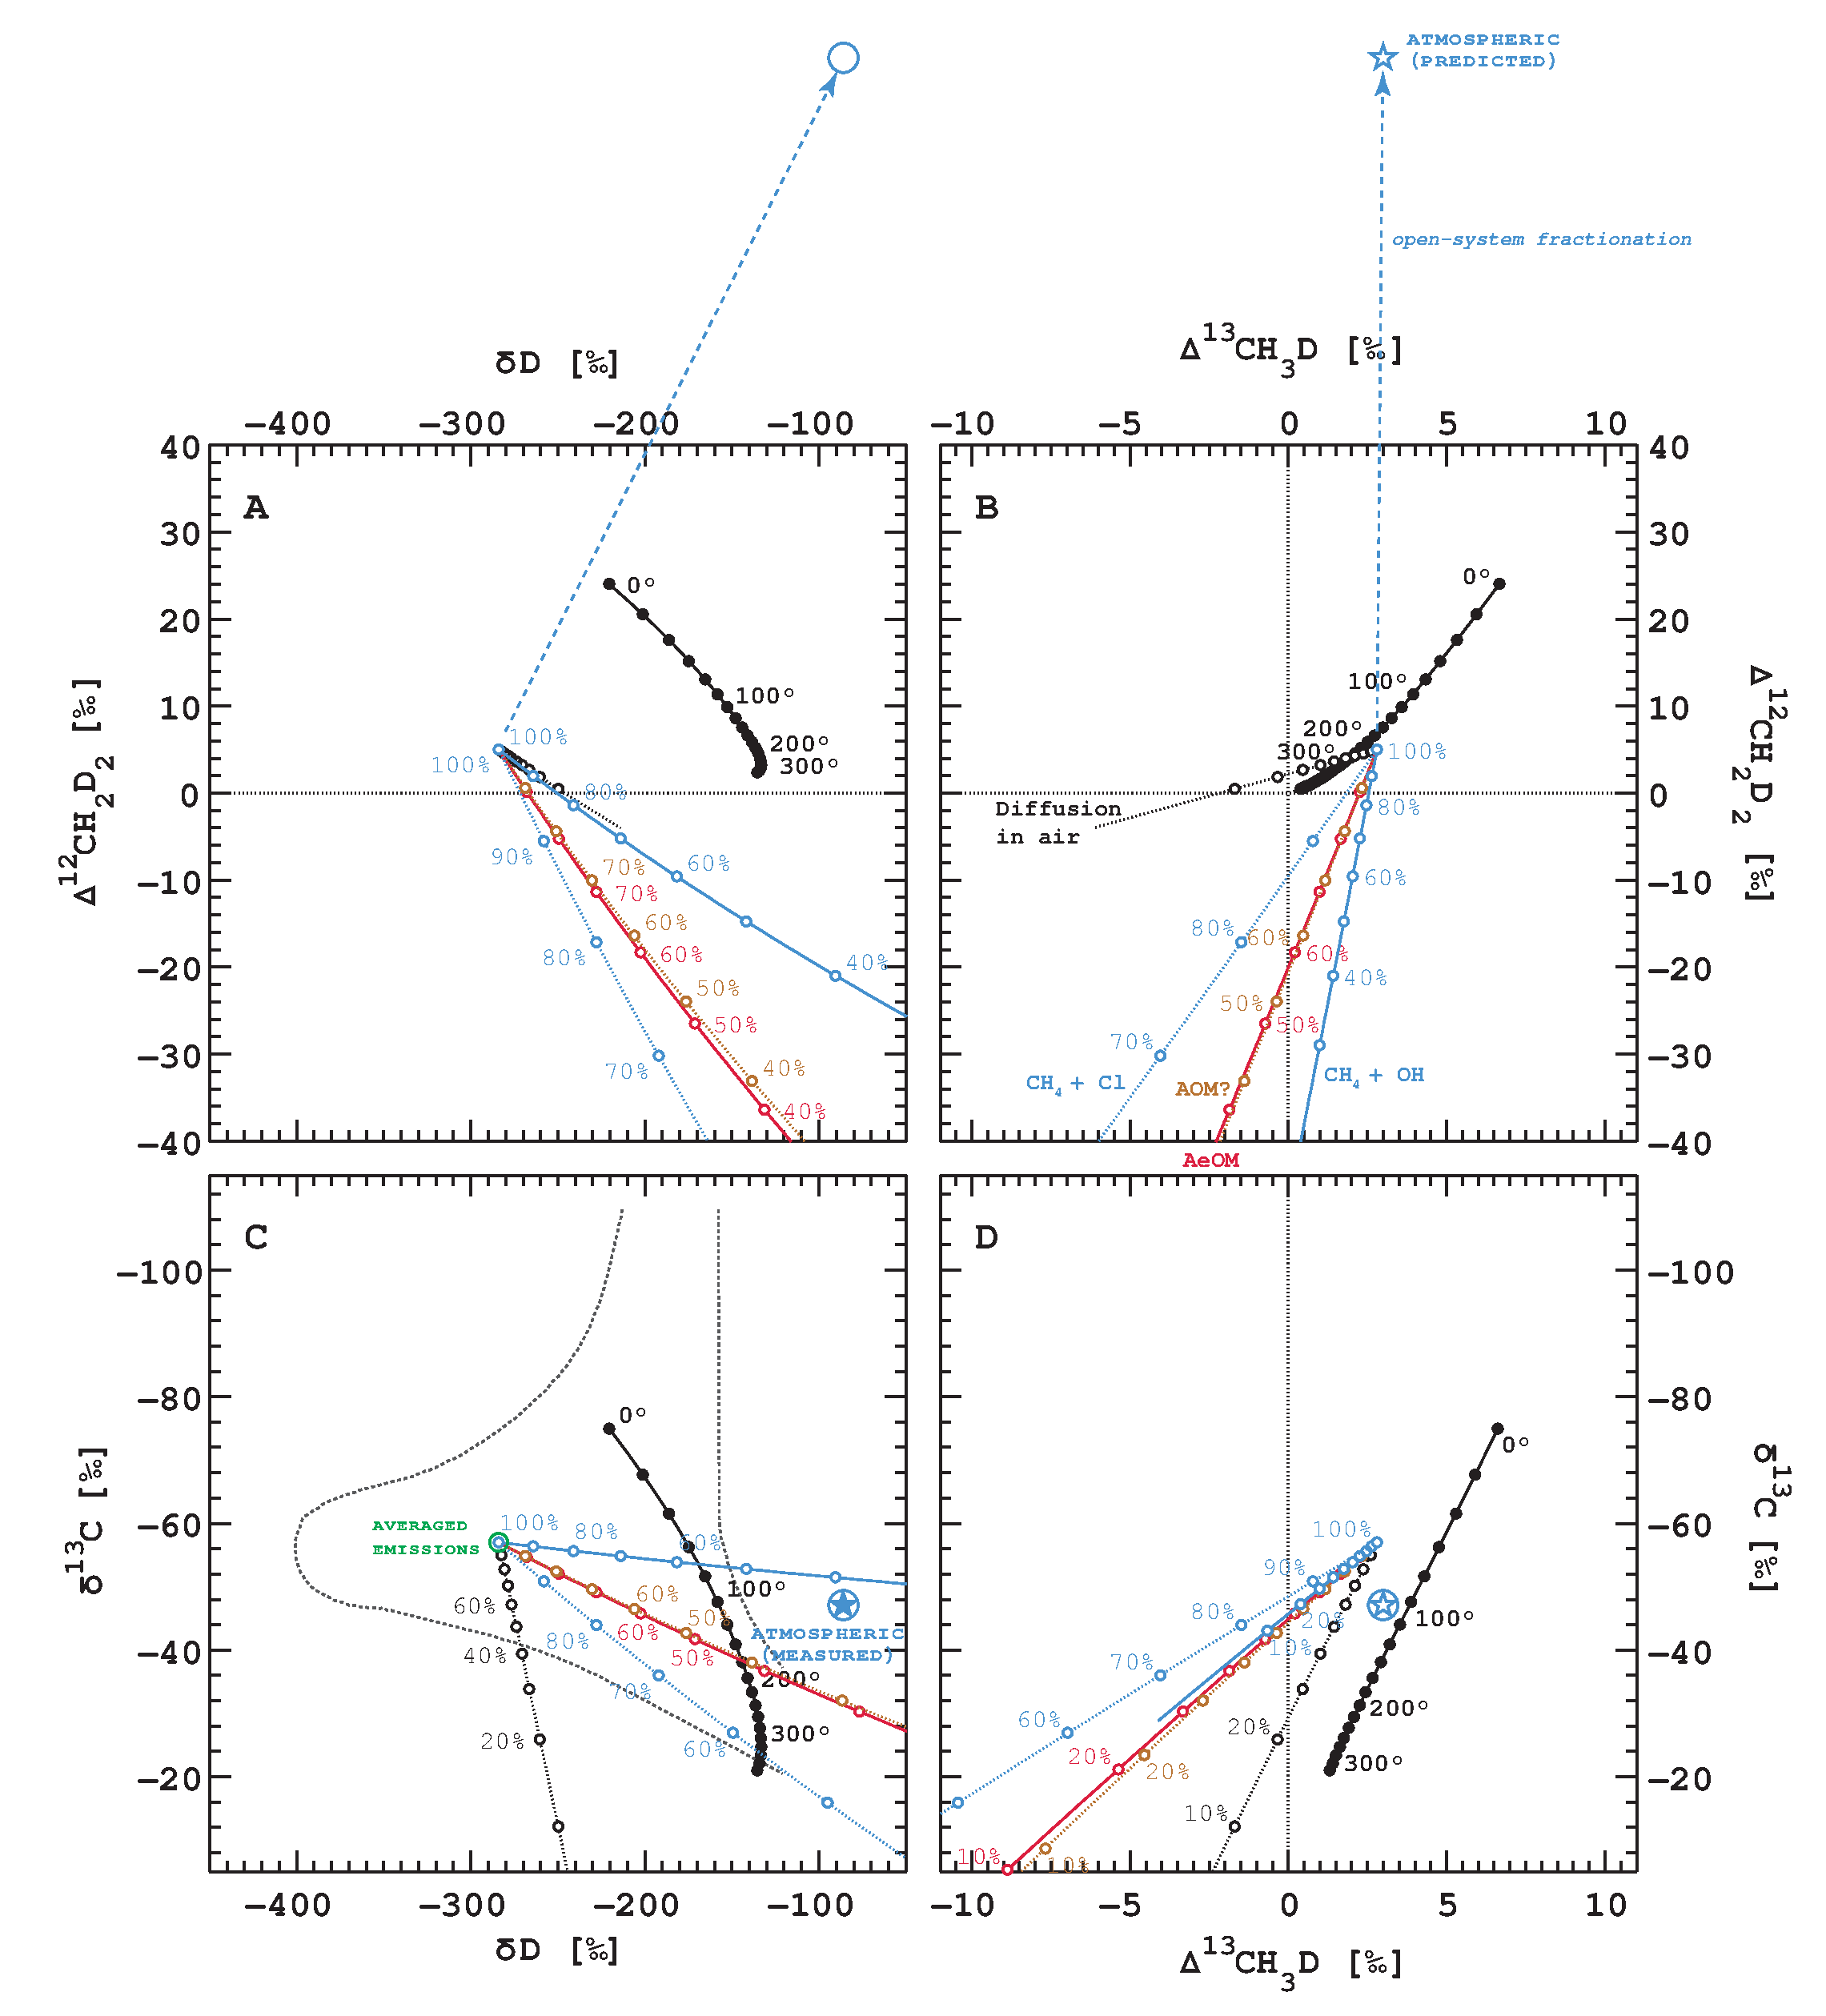
\includegraphics[scale=0.42]{figures/Fig5.5.pdf}
%	\captionsetup{format=myformat}	% hrule beneath caption
	\caption[Behavior of methane isotopologues during methane breakdown]{Evolution of CH\textsubscript{4} isotopologue ratios in
		closed-system, unidirectional bond-breaking processes. Predictions are
		derived from models and/or data presented by the MIT and UCLA teams
		\parencite{Wang++_2016_GCA,Whitehill++_2017_GCA,Young++_2017_GCA}.
		Calculations used the estimated weighted average of modern sources of
		atmospheric methane as the starting point. Trajectory labels indicate
		the fraction of remaining CH\textsubscript{4}. Predictions of
		atmospheric Δ\textsuperscript{13}CH\textsubscript{3}D and
		Δ\textsuperscript{12}CH\textsubscript{2}D\textsubscript{2} assume an
		open system in steady-state. Note that partial reversibility of the
		depicted processes will tend to pull the vectors towards the equilibrium
		line.}
	\label{fig:5:5}
\end{figure*}




